\section{Controlling a Superconducting Quantum Computer} \label{chap:FPGA}
\subsection{Overview}
Before jumping into the specifics of how'd we control the quantum computer, let's start with a general overview and show how everything is connected.

This is a diagram that shows how the system is connected, from the pulse generator to the cavity.

\begin{figure}[H]
    \centering
    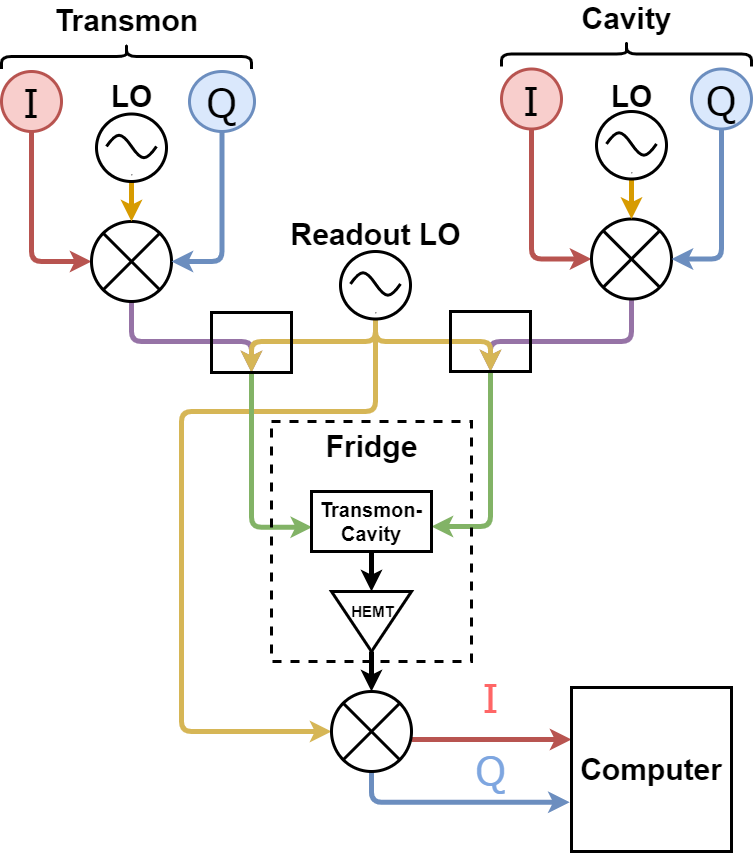
\includegraphics[width=0.85\columnwidth]{overview.png}
    \caption{Diagram of the system}
    \label{fig:System-diagram}
\end{figure}

The $I$ and $Q$ signals are generated in the AWG, the LO frequency comes from a frequency generator and so does the Read Out signal. \textbf{H}igh \textbf{E}lectron \textbf{M}obility \textbf{T}ransistor (HEMT) is a low-noise cryogenic amplifier.

\subsection{Generating the Pulses}
\subsubsection{The AWG}
% It shouldn't be too much of a surprise if I'll tell you that I consider the AWG (Arbitrary Waveform Generator) the "heart\ensuremath\heartsuit" of the system, we've just spent an entire chapter on finding the pulses we want to send, and the instrument that creates and sends the pulse, is the AWG. Unfortunately, using the AWG isn't as straight-forward as you might hope and there are some problem's we'll need to address if we want our system to work.

An \textbf{A}rbitrary \textbf{W}aveform \textbf{G}enerator (AWG) is a device that we use to generate the pulses we calculated with GRAPE in the previous chapter. To control the qubit we need to send RF signals, typically ranging from $4$GHz to $10$GHz. Such signals can be generated by RF signal generators (also called LO's - local oscillators). In contrast, the AWG sends out slowly varying envelopes, usually with a bandwidth of a few hundred MHz. To bridge this gap, we will mix a fixed-frequency signal from the LO with a time-varying signal from the AWG. In particular, this will also enable us to vary the frequency of the LO in real-time with the AWG. Our goal in the next section will be to achieve this so called single-sideband modulation of the LO signal.

We also want to be able to un-mix the measurement result to get back only the interesting parts of the pulse. The device we'll use for this task is the \textit{IQ-Mixer}, but before we can  get into the IQ-Mixer, we need to understand how a \textit{regular} mixer works.

\subsubsection{The Mixer}
The mixer has 2 inputs and one output. When you enter 2 pulses as an input, you get their product as the output (inputting for example $\cos (t)$ and $\cos (2t)$ will result in $\cos (t)cos (2t)$ at the output).
We draw a mixer in a diagram as
\begin{figure}[H]
    \centering
    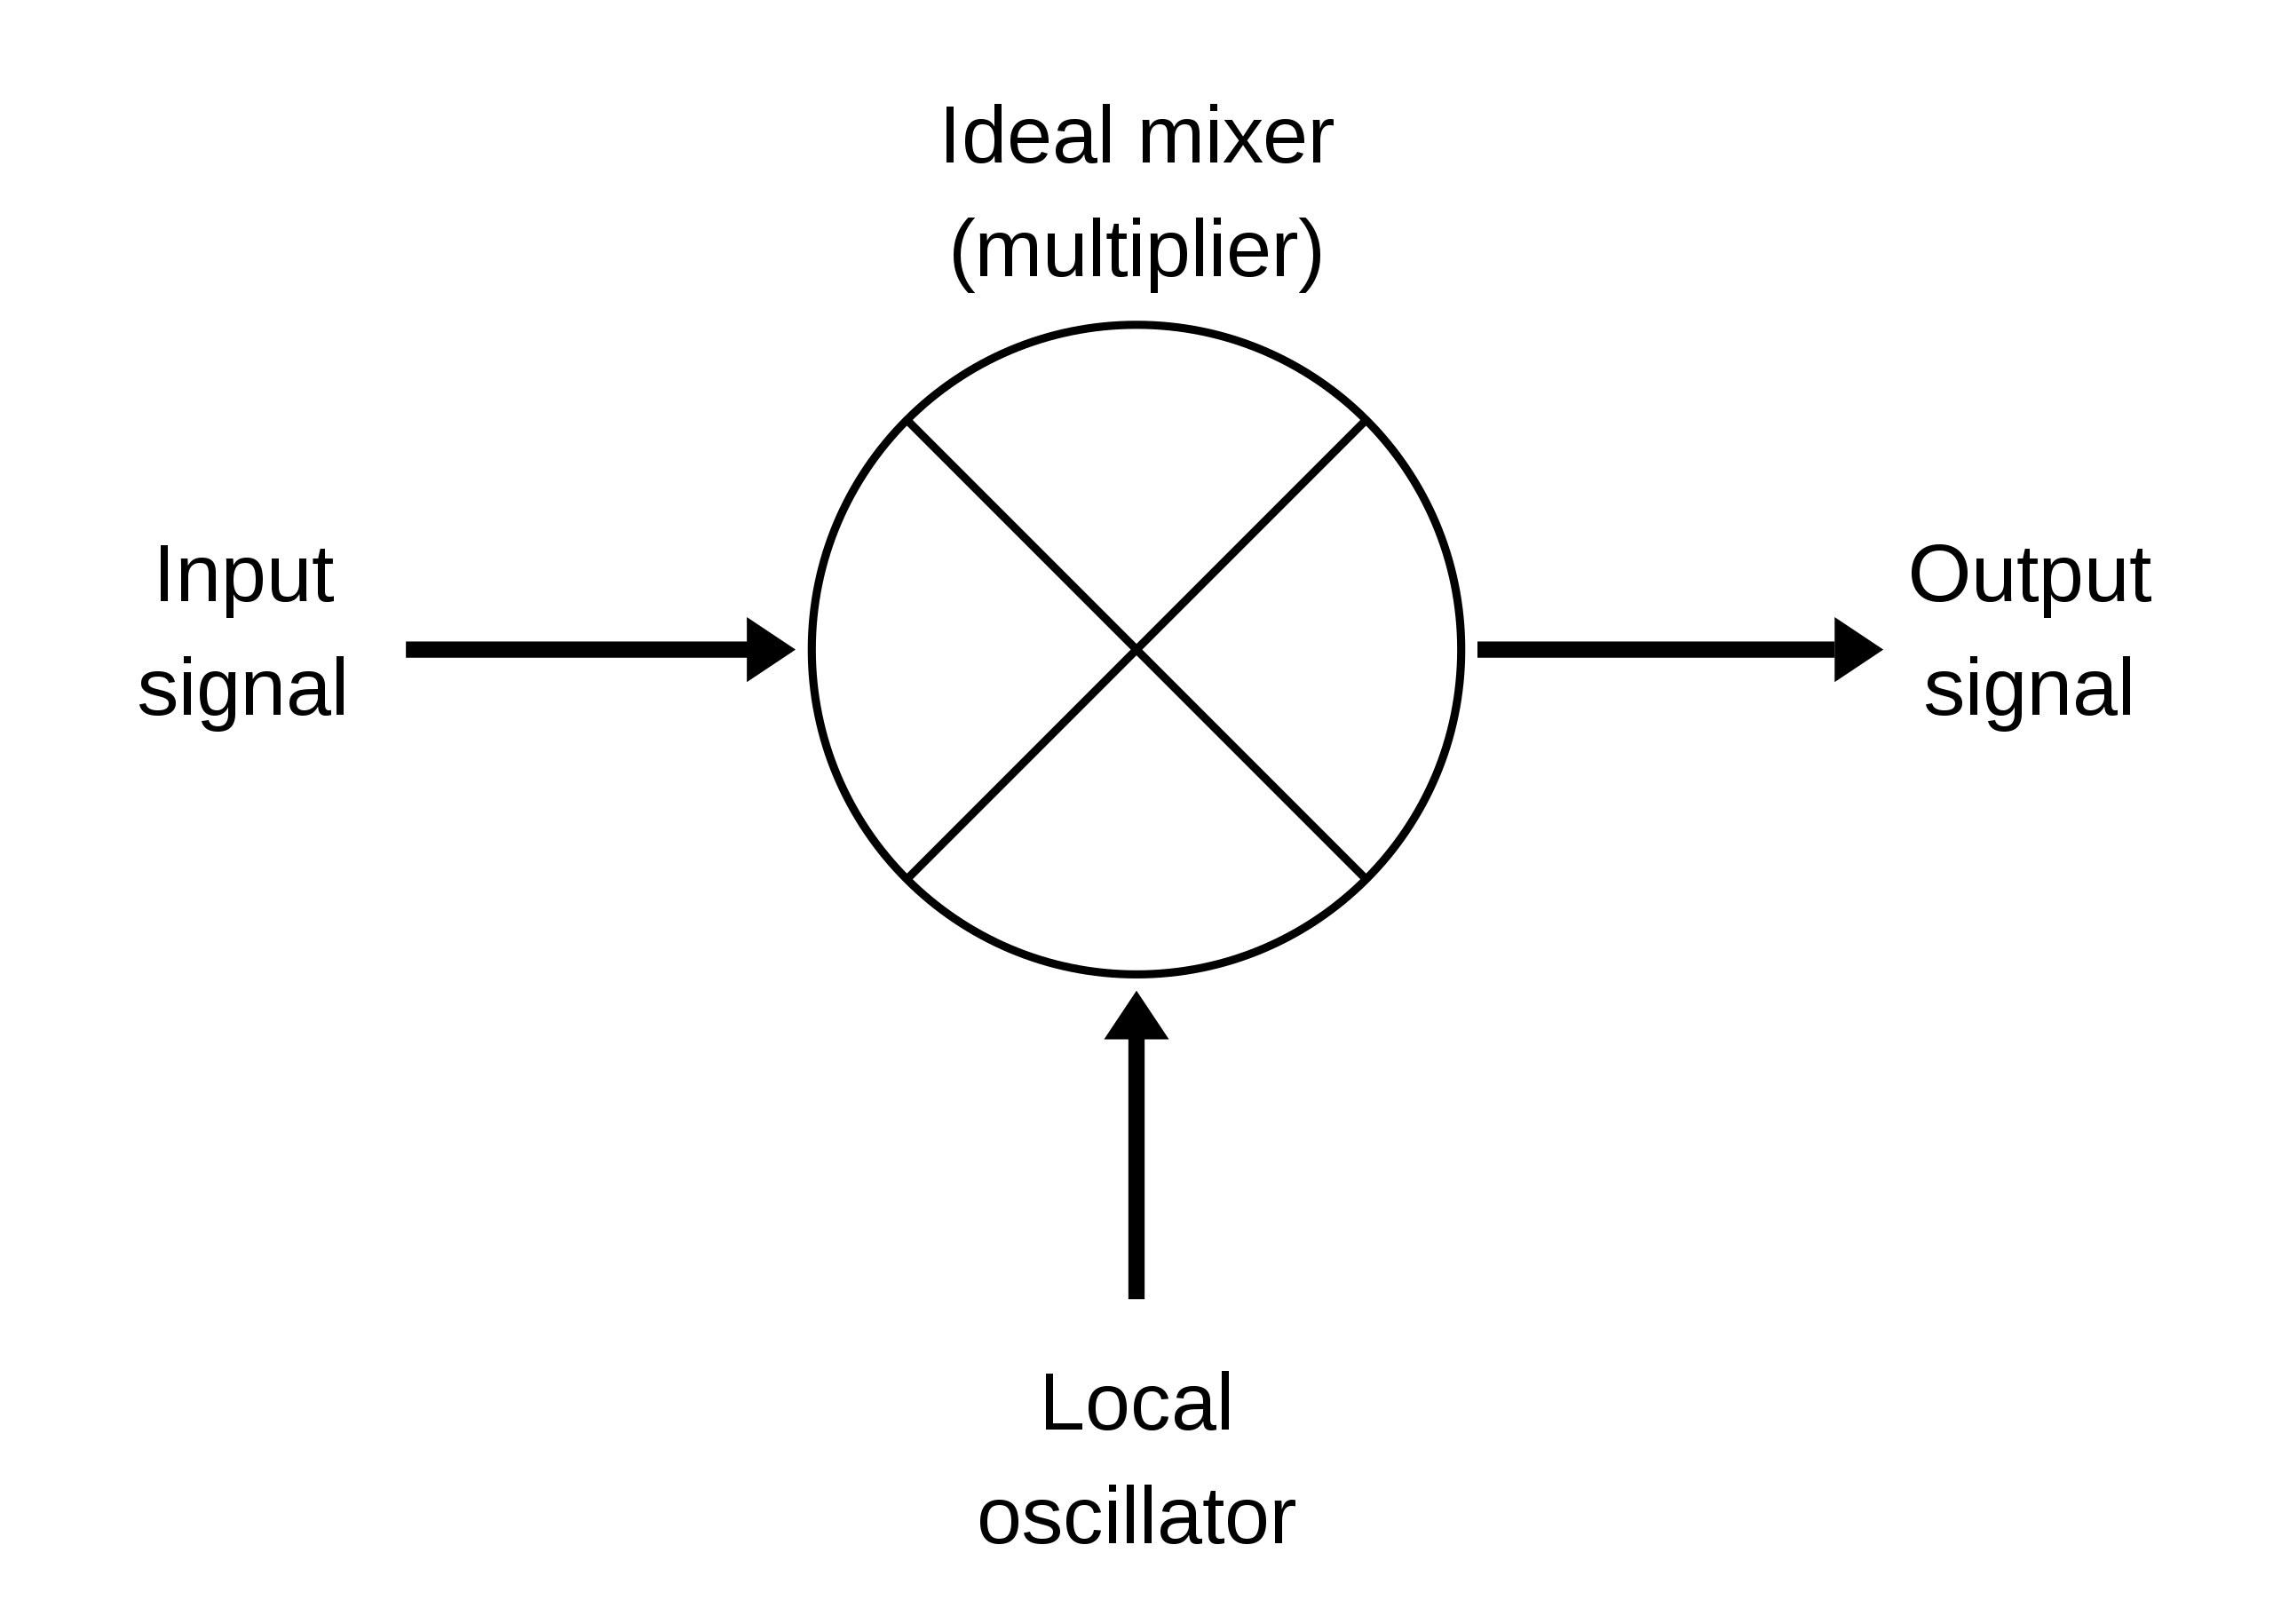
\includegraphics[width=0.3\columnwidth]{Ideal-Mixer.png}
    \caption{Ideal mixer in a diagram}
    \label{fig:Ideal-Mixer}
\end{figure}
The mixer circuit is \textit{non-linear}. The non-linearity could be achieved with non-linear components, such as diods.
% We can change what are the outputs and what are the inputs to get different ways for the mixer to work\footnote{TODO: Explain this} % TODO: Add on this later

\subsubsection{The IQ-Mixer}
We've seen what's a \textit{regular} (and \textit{ideal}) mixer is, but how can we use it for the desired effect? remember, we want to input a high frequency and a lower frequency and we want the output to be a wave with a frequency that is the sum of the 2 frequencies. To do so, we can consider the following diagram
\begin{figure}[H]
    \centering
    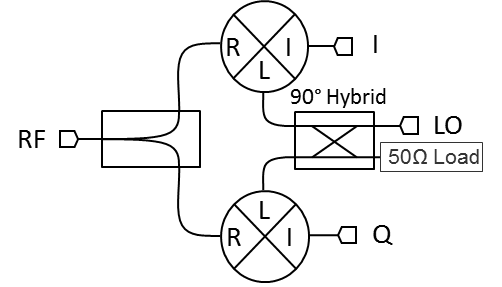
\includegraphics[width=0.5\columnwidth]{IQ-Mixer.png}
    \caption{The IQ mixer}
    \label{fig:IQ-Mixer}
\end{figure}
Where the 90\degree\ hybrid in the diagram is a \textit{90\degree\  hybrid coupler}. This device splits the signal into 2 signals at a 90\degree phase difference, hence the name. The square near the \textit{RF} sign simply adds the 2 waves.

As we can see, the IQ mixer has 3 inputs, In-phase (\textit{I}), Quadrature (\textit{Q}), hence the name, and \textit{LO}. We can also see that there's only one output, \textit{RF} (although you can reverse the roles of the input and the output).

How can we use this IQ mixer to add frequencies? Let's consider the following inputs\footnote{You can flip I and Q and get subtraction instead of addition}
\begin{align*}
    I &---> \cos (\omega_{IQ} t)\\
    Q &---> \sin (\omega_{IQ} t)\\
    LO &---> \sin (\omega_{LO}t)
\end{align*}
In this case, the input into the top mixer will be \textit{I} and a \textit{LO}, which is $\cos (\omega_{IQ}t)\sin (\omega_{LO}t)$. Similarly, the input into the bottom mixer will be \textit{Q} and 90\degree phase of \textit{LO}, which is $\sin (\omega_{IQ}t)\cos (\omega_{LO}t)$.

The total output (in \textit{RF}) will be the sum of the two waves
$$RF = \cos (\omega_{IQ}t)\sin (\omega_{LO}t) + \sin (\omega_{IQ}t)\cos (\omega_{LO}t)$$
So we get
\begin{equation}
    \boxed{RF = \sin ( (\omega_{LO} + \omega_{IQ})t)}
\end{equation}

Perfect! this is exactly what we wanted, the output is a wave with frequency that is the sum of the input frequencies. Only one problem, this simple scheme turns out not to work in practice : (.

\subsubsection{Theory VS Reality} \label{sec:solution_real_world} % Maybe combine this section and the next one
If we use a spectrum analyzer and view what frequencies are in the final wave we get the following picture

\begin{figure}[H]
    \centering
    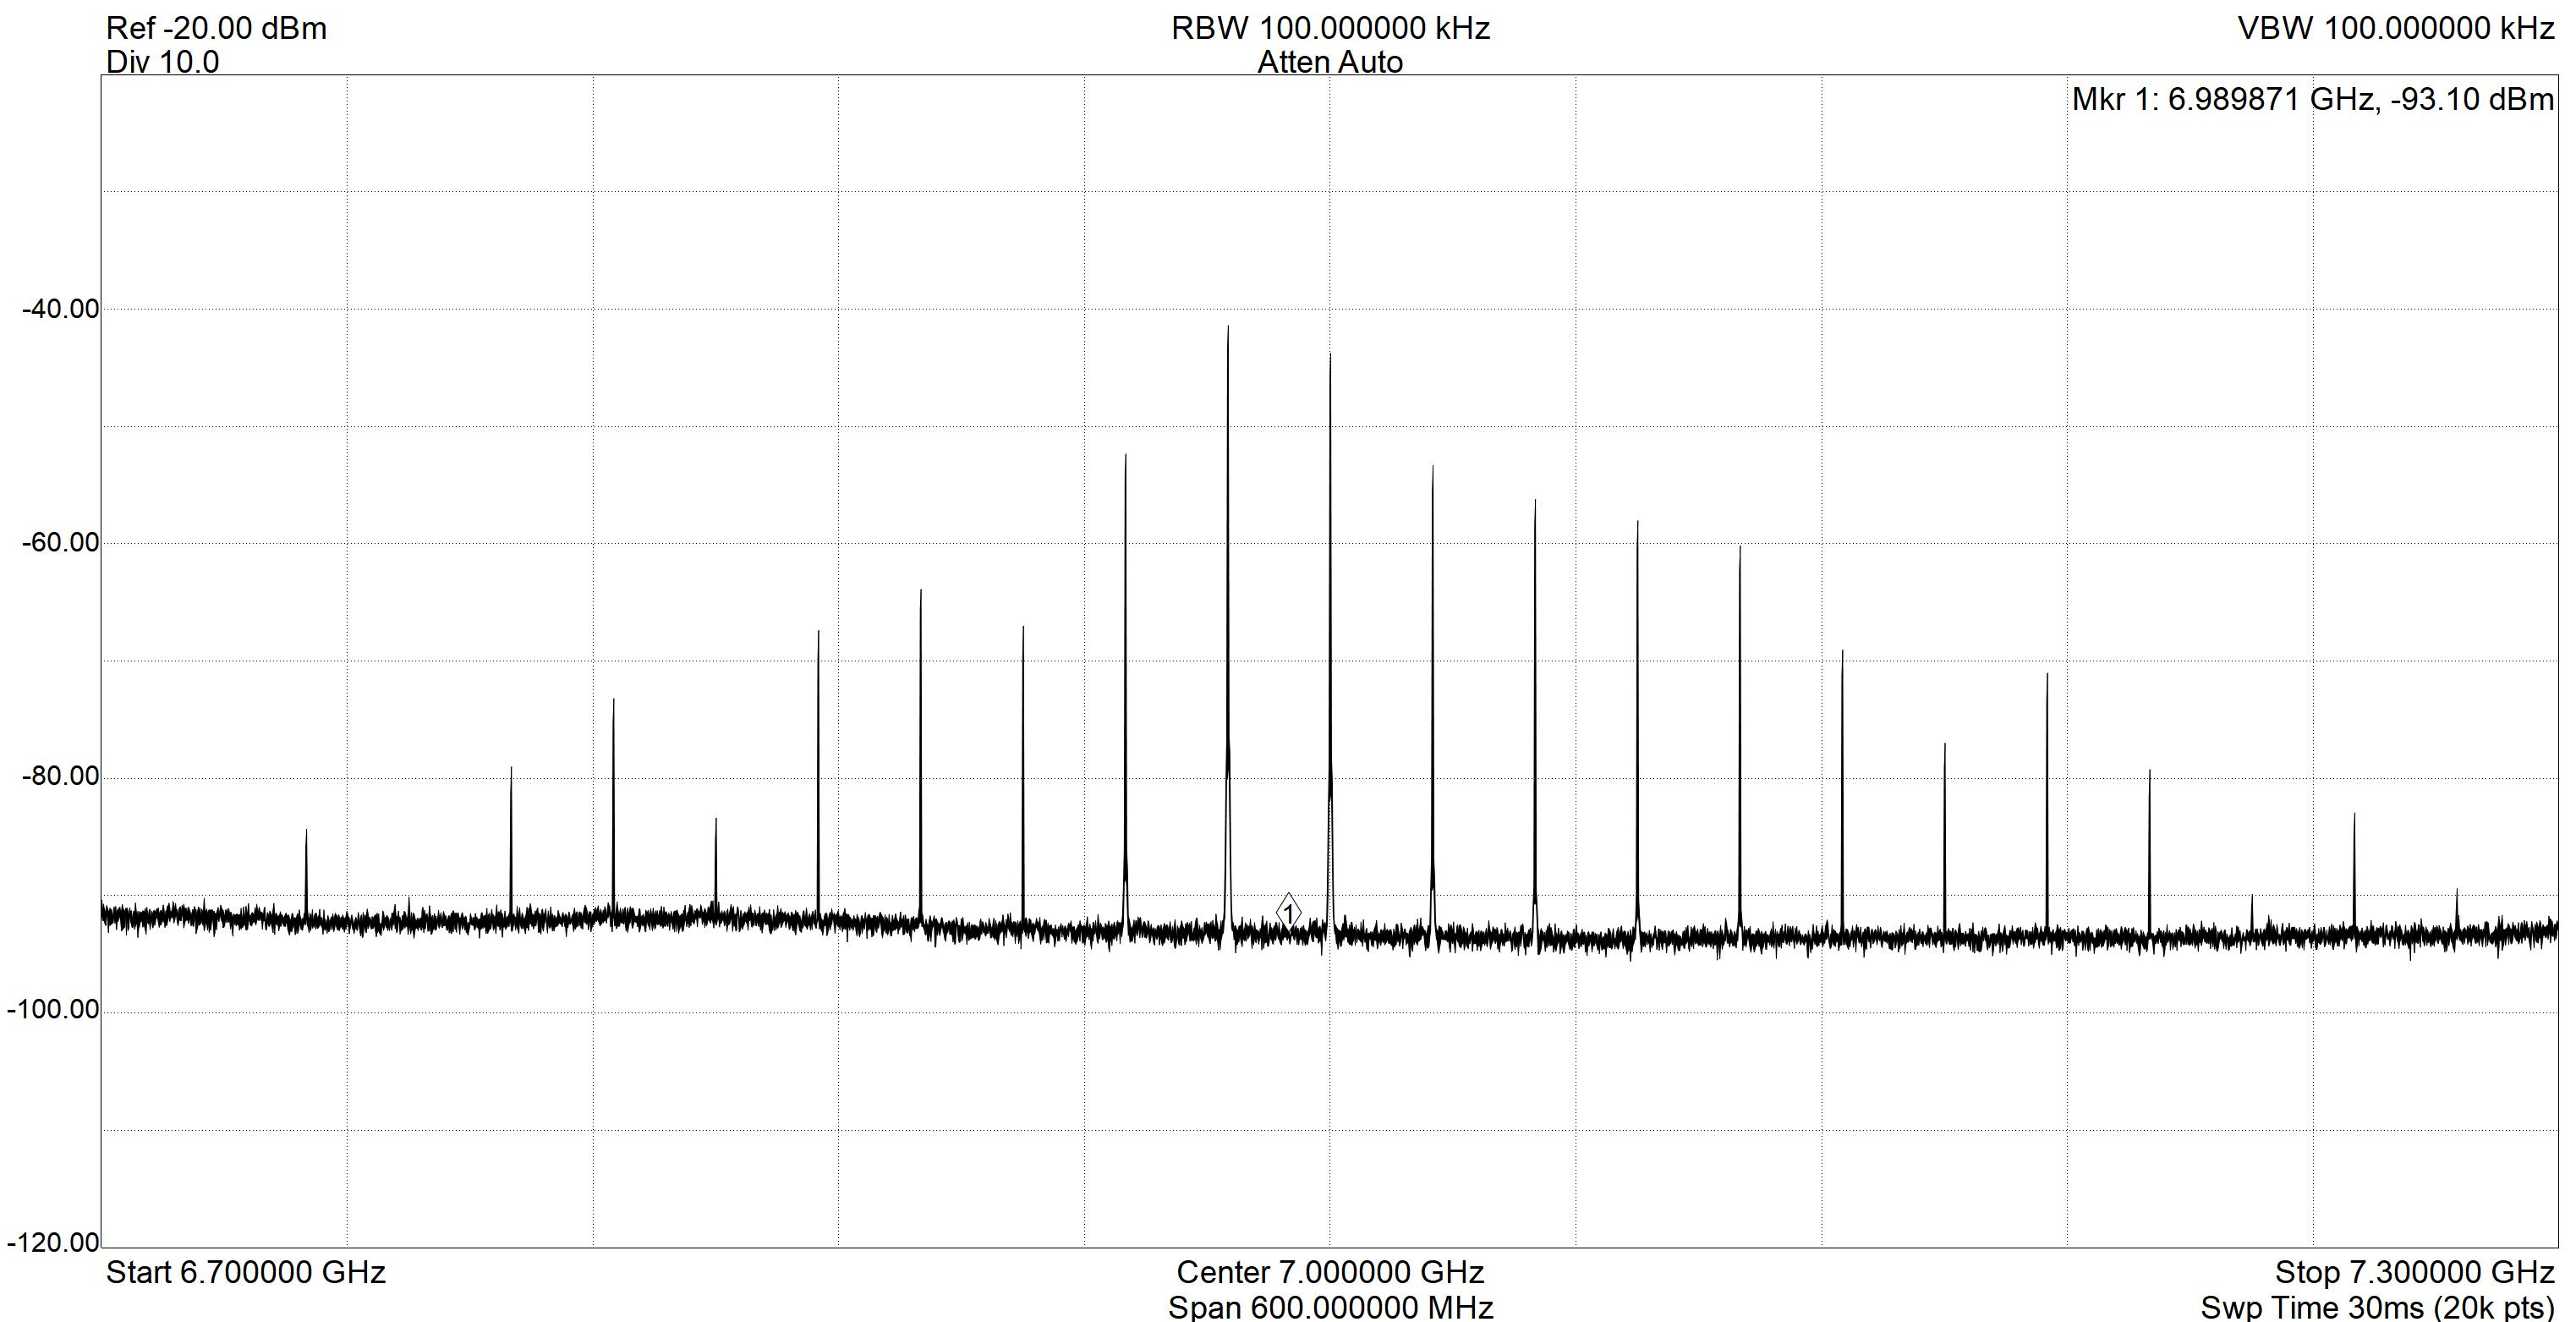
\includegraphics[width=0.8\columnwidth]{full-spectrum-no-correction.jpg} %TODO: Need to change to image with explantion on what is going on
    \caption{Full Spectrum Without Any Corrections}
    \label{fig:Full-spectrum-no-corrections}
\end{figure}
Zooming in around the LO frequency we see
\begin{figure}[H]
    \centering
    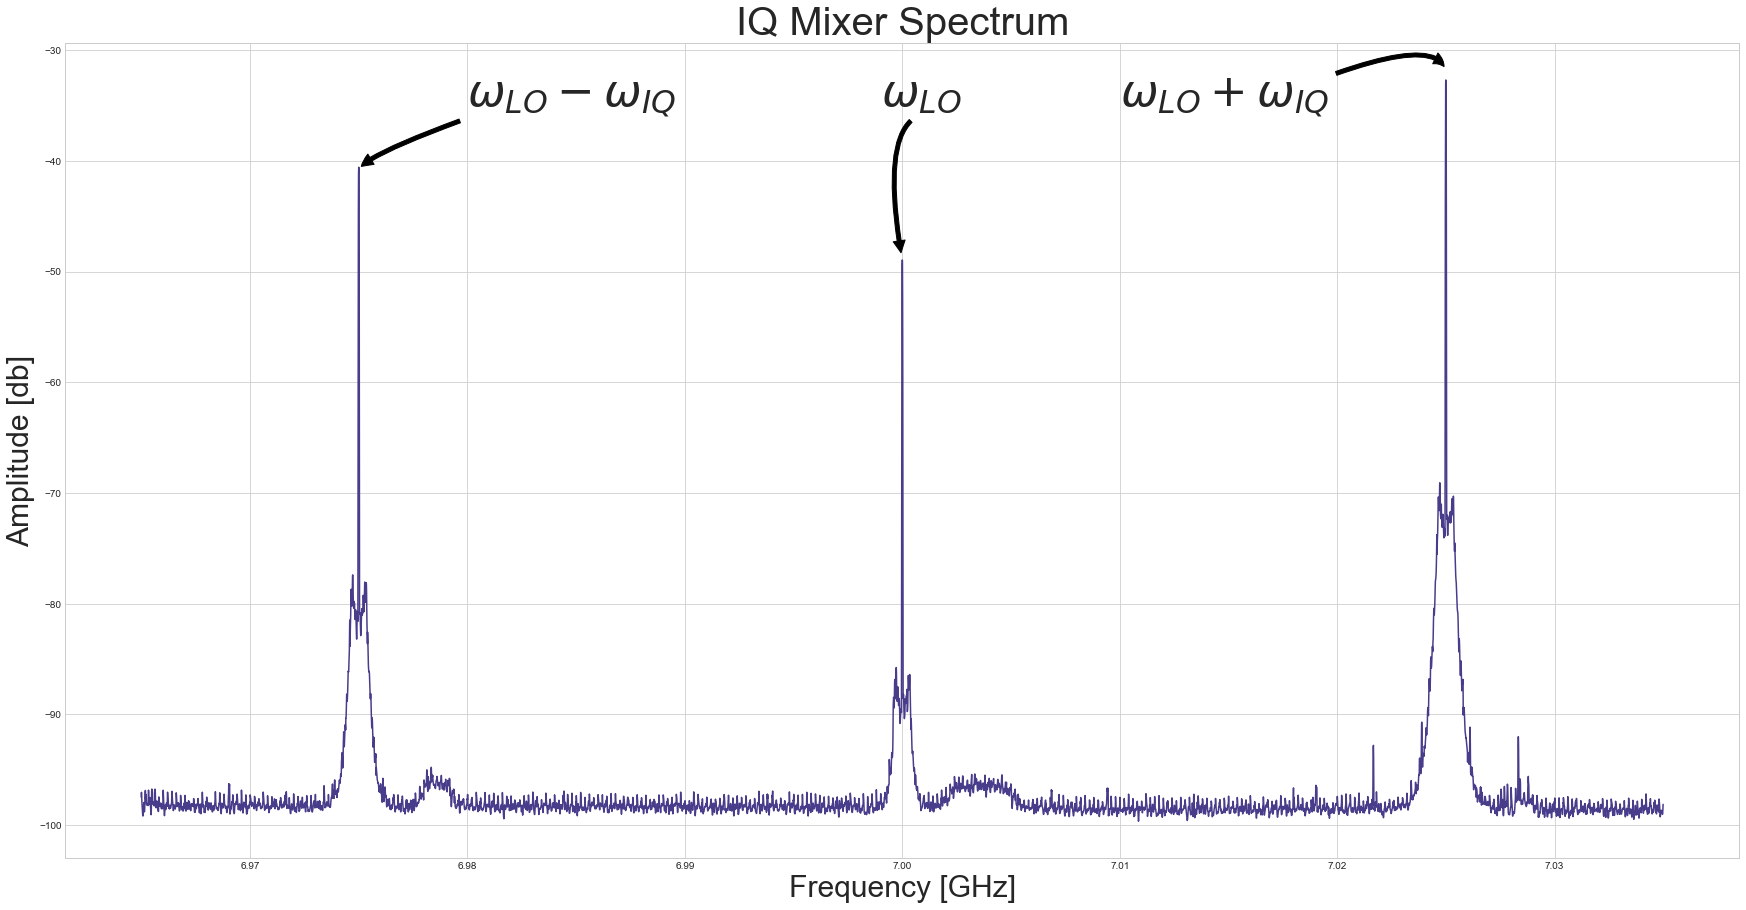
\includegraphics[width=0.9\columnwidth]{Important-Spectrum-no-correction2.png} 
    \caption{Spectrum Around the LO Frequency}
    \label{fig:closeup-spectrum-no-corrections}
\end{figure}

What is the problem? We've proved mathematically that it should work, so why doesn't it? The problem is that we can't just assume the waves to come and go with the same phase, the waves travel through the wire at some speed so if we input into two different wires, two waves that are at the same phase, at the other side of the wire they might come at different phases because of differences in wire length, resistance, etc... So what can we do about it? You could try to make identical parts and make everything just perfect but even slight deviation will cause the system no to work properly, a better solution is to input more complex waves and have some parameters to play with so we can simply find the right parameters for the system.% TODO: Improve wording

We can analyze the frequency space of the output of out IQ mixer and we can see two types of it not working correctly
\begin{itemize}
  \item Leakage at the LO frequency
  \item Leakage at the sideband ($\omega_{LO} - \omega_{IQ}$)
\end{itemize}
We can solve the first type of Leakage, at the LO frequency, by adding DC offsets to the input frequencies (We'll prove this mathematically later), and we can solve the second type of leakage by adding phase offsets to the waves (We'll prove this mathematically later).
% This is how the frequency spectrum looks without making any changes to the input waves


% \subsubsection{Solution for the real world} \label{sec:solution_real_world}
Before we can solve the problem, we need to understand what's causing it. As we explained earlier, a phase  is created  in the wires that connect everything.
\paragraph*{Leakage at $\omega_{LO} - \omega_{IQ}$ }
% \subsection{What's causing the problem}
Let's consider now inputting into the IQ mixer the same waves but with the phases that were created in the transmission wires instead of what we had earlier
\begin{align*}
    I &---> \cos (\omega_{IQ} t + \phi_I) \\% + \epsilon_I\\
    Q &---> \sin (\omega_{IQ} t + \phi_Q) \\% + \epsilon_Q\\
    LO &---> \sin (\omega_{LO}t + \phi_{LO})
\end{align*}
Using the same calculation we did before, we get that
$$RF = I\cdot LO + Q\cdot LO (90\degree)$$
\[
RF = \cos (\omega_{IQ} t + \phi_I) \cdot \sin (\omega_{LO}t + \phi_{LO}) + \sin (\omega_{IQ} t + \phi_Q) \cdot \cos (\omega_{LO}t + \phi_{LO}) 
\]
After some algebra we get
\begin{align*}
RF = &\cos (\frac{\phi_Q - \phi_I}{2})\sin ( (\omega_{IQ} + \omega_{LO})t + \frac{\phi_Q + \phi_I}{2} + \phi_{LO}) \\
   + &\sin (\frac{\phi_Q - \phi_I}{2})\cos ( (\omega_{IQ} - \omega_{LO})t + \frac{\phi_Q + \phi_I}{2} - \phi_{LO})
\end{align*}
This expression is quiet scarier than the one we got earlier... More than that, we get two frequencies instead of one, we've got an unwanted frequency at $\omega_{LO} - \omega_{IQ}$ and the only way to make it disappear is if the phases are equal, $\phi_I = \phi_Q$. Also the final wave as a phase of $\phi_{LO}$, this isn't really a problem and if we define our starting point differently we can set  $\phi_{LO}$ to 0.

\paragraph*{LO Frequency Leakage}
% TODO: Maybe I'll be able to find a mathematicall explenation to the DC offsets
Another type of leakage we've observed is leakage at the LO frequency, it makes sense that some of the original wave will go through the mixer untouched. To fix that leakage, we'll need to somehow change the I and Q waves to cancel it out. The simplest way to do so is to add DC offsets to the inputs \footnote{I've removed the phase on the LO wave since we've seen it doesn't really change anything}
\begin{align*}
    I &---> \cos (\omega_{IQ} t + \phi_I) + \epsilon_I\\
    Q &---> \sin (\omega_{IQ} t + \phi_Q) + \epsilon_Q\\
    LO &---> \sin (\omega_{LO}t)
\end{align*}
We've seen this story before... the calculation of the RF wave is the same so we'll skip the calculation. The end result is
\begin{align*}
RF = &\cos (\frac{\phi_Q - \phi_I}{2})\sin ( (\omega_{IQ} + \omega_{LO})t + \frac{\phi_Q + \phi_I}{2}) \\
   + &\sin (\frac{\phi_Q - \phi_I}{2})\cos ( (\omega_{IQ} - \omega_{LO})t + \frac{\phi_Q + \phi_I}{2}) \\
   + &\epsilon_I  \sin (\omega_{LO}t) + \epsilon_Q  \cos (\omega_{LO}t) \\
   = &RF_{old} + \epsilon_I  \sin (\omega_{LO}t) + \epsilon_Q  \cos (\omega_{LO}t)
\end{align*}
where $RF_{old}$ is the RF wave before adding the DC offsets. 

What we get is the same wave, but now we can play with the LO frequency at the output. Later we'll change the DC offsets so that they will cancel to LO frequency leakage to minimize it.

Now that we have all of our "knobs" we can change and play with, we can start using them to minimize the leakages.


\subsubsection{Finding Optimal Constants} % Maybe I won't do this section
As we've seen in the previous section, there are 4 variables we can "play" with to get the best variables for our system, as long as we don't change the system, these variables stay the same. What we want to do now is to actually find them. Our system is connected like so
% Add figure of how the system is connected

We have the Quantum Machine\footnote{this is the heart of the system, for now we'll use it to make the MHz waves with different phases, DC offsets and frequencies} that generates the I and Q inputs that go into the mixer (and also to an oscilloscope for debugging). There's the frequency generator\footnote{KeySight N5173B} that is connected to the mixer and generates 7GHz wave, and there's the frequency spectrum analyzer\footnote{SignalHound USB SA-124B} that is connected to the computer.

Let's first attack the leakage at the LO frequency. For now we'll have an LO frequency of 7GHz that we want to change by 25MHz (The same variables work for all frequencies this is just as an example)

\paragraph{LO frequency Leakage}
As proven in section \ref{sec:solution_real_world}, to minimize this kind of leakage all we need is to play with the DC offsets of the IQ inputs. To do so, we first need to define what we want to minimize, which in this case is simply the power of the frequency at 7GHz, we can measure that power with our spectrum analyzer, we'll call that our \textit{cost function}.
We have a 2-dimensional variable space, we need to find where in this space the cost function is at a minimum. To do so, we'll start by using a brute force method to find the general location of the minimum in the variable space, since brute force is very inefficient we can't really use it to find the exact location of the minimum so we start by only doing a low precision brute force and then use a different optimization algorithm to find the exact location of the minimum. We'll use the \texttt{scipy.optimize.fmin} as the algorithm for precise minimum location.
% TODO: Add figure of spectrum after leakage optimazation, Improve wording

\paragraph{Sideband Leakage}
Now that we've minimized the LO frequency leakage, we want to minimize the sideband leakage. We do that by changing the phases of the IQ waves from the quantum machine, it's important that changing the phases doesn't change the LO leakage and luckily for us, as proven in section \ref{sec:solution_real_world} that's whats happening. to change the phases we don't simply specify the phases, we use the correction matrix of the Quantum Machine.
This time our cost function is the frequency at $\omega_{LO} - \omega_{IQ}$, we can do the same as we did in the LO leakage and use first a brute force optimization to find the general location of the minimum and the use the fmin algorithm to find the exact location of the minimum of the cost function (this time in the scale-angle variable space). You can see the result here
% TODO: Add figure of full final optimization, Explain why it doesn't work perfectly (The quantum machine power problem)
\begin{figure}[H]
    \centering
    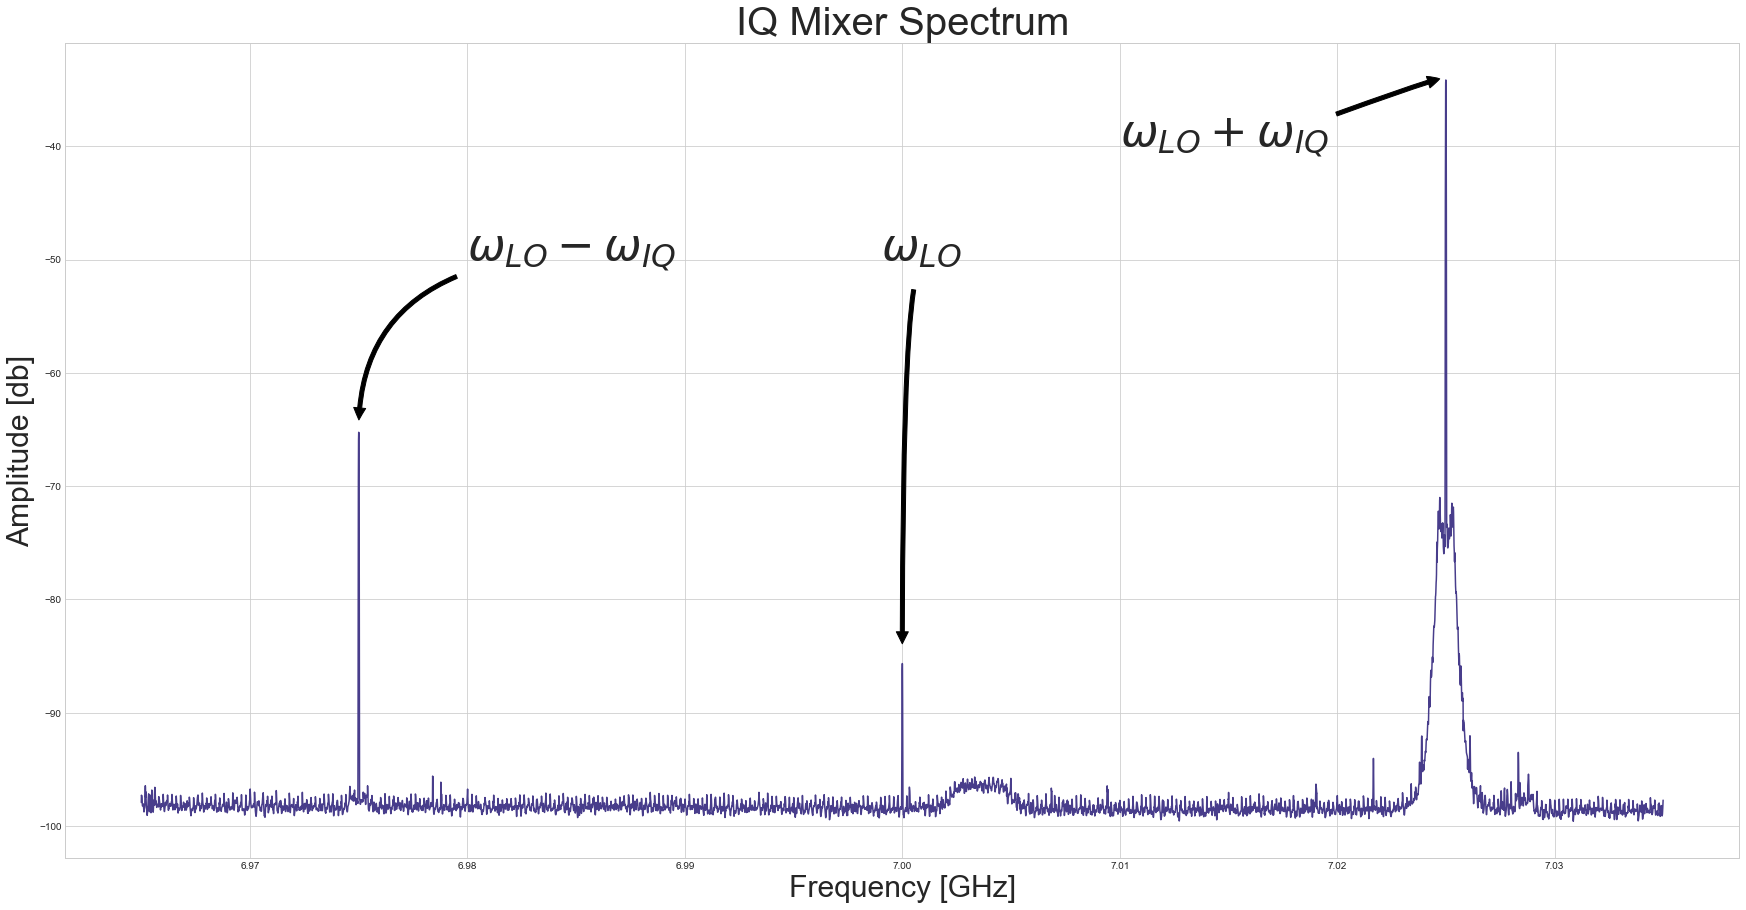
\includegraphics[width=0.9\columnwidth]{Important-Spectrum-all-correction2.png} 
    \caption{Spectrum Around the LO Frequency}
    \label{fig:closeup-spectrum-no-corrections}
\end{figure}
The other frequencies aren't completely reduced because nothing is perfect, but ir's pretty close and good enough for this demonstration.

\subsection{References and Further Readings}
A great book on couplers and mixers I used while writing this chapter is "\textbf{Microwave Engineering}" by David M. Pozar. It provides a much more in depth look on the subject.

Another great resource is the \textbf{Marki Microwave RF \& Microwave knowledge base} at \newline \texttt{https://www.markimicrowave.com/engineering/}. Which provides useful introduction to many topics in microwave engineering.